% main.tex, to be used with thesis.tex
% This contains the main work of your thesis.

%\bibliography{thesis}  % uses the references stored in Chapter1Radar.bib

\chapter{Data Persistence Technology for Sensor Networks: An Empirical-based
Choice for NetBEAMS}

This chapter analyzes each of the taxonomies defined in chapter
\ref{chap:taxonomies} against the requirements defined by our case study,
NetBEAMS, in chapter \ref{sec:problem-requirements}. Moreover, it evaluates
different database technologies against on those taxonomies, and tries to select
one of them which can be a candidate for an experimental analysis.

First, the contender technologies are as follows:

\begin{itemize}
  \item MySQL
  \item Microsoft SQL 
  \item Berkeley TinyDB
  \item MongoDB
  \item CouchDB
  \item IBM DB2
\end{itemize}


\section{Analysis of the Purpose of Sensor Data Taxonomy}

Considering the infrastructure of NetBEAMS, as described in the previous
chapter, and the characteristics of the sensor network defined at the SF-BEAMS
\cite{sfbeams2006} site, the data characteristics are as follows:

\begin{itemize}
  \item Data is generated by sensor devices, such as the YSI sonde
  \cite{YSI-Sonde}, and manually collected by using a laptop to the network
  sink at the RTC laboratories;
  \item Upon data reception, the RTC staff index and archive the data for
  for distribution using the OPEnDAP format;
  \item Another approach for data collection of data generated by the SF-BEAMS
  is the use of NetBEAMS \cite{netbeams2009}, as described in section
  \ref{netbeams-architecture}.
\end{itemize}

Given the facts collected from the observations of the execution of NetBEAMS
through the SF-BEAMS sensor network, we can say that the purpose of collected
data is \textbf{Data Archival}.

\subsection{Technology Analysis}

Any of the contenders are options to cover for Data Archival.

\begin{itemize}
  \item \textbf{MySQL}: Supports
  \item \textbf{Microsoft SQL}: Supports
  \item \textbf{Berkeley TinyDB}: Supports
  \item \textbf{MongoDB}: Supports
  \item \textbf{CouchDB}: Supports
  \item \textbf{IBM DB2}: Supports
\end{itemize}

\section{Analysis of the Location of Sensor Data Taxonomy}

Some observations regarding the location of the collected sensor data for
NetBEAMS were described in the previous section and summarized as follows:

\begin{itemize}
  \item NetBEAMS's architecture is based on a single-hop star infrastructure 
   with a direct network sink being the RTC server \ref{sec:sn-infrastructure}.
\end{itemize}

Based in the observations described, the type used for storing
data can be either the \textbf{External Storage} or the
\textbf{Data-Centric Storage}. The former is the current approach used by the
SF-BEAMS sensor network, while the latter adopted as an improvement of the
persistence infrastructure for NetBEAMS.

\subsection{Advantages of the External Storage Approach}

The External Storage approach is the most common way to implement persistence
for any type of systems, including sensor networks, due to its the simplistic
data management. Furthermore, this type of setup is easier to use of
distributed systems approaches such as Replication to help preventing scaling
the system.

\subsection{Disadvantages of the External Storage Approach}

The most common problem related to a single External Data Storage is that
resources may run into data management problems such as full disk space or disk
failures.

\subsection{Advantages of the Data-Centric Approach}

The advantage of the Data-Centric approach lies on the way that data is
distributed into different locations. By using techniques of distributed
database systems, the approach improves overall performance of the use of
massive data sets since the operations of the data are directed to specific
locations. Besides, this approach helps the network managers scale the data
storage just by adding new data nodes as required.

\subsection{Disadvantages of the Data-Centric Approach}

The data partitioning is a very restricted technology, mostly available to
advanced users of distributed database systems. The main users of wireless
sensor networks do not have such expertise.

\subsection{Technology Analysis}

\begin{itemize}
  \item \textbf{MySQL}: Supports
  \item \textbf{Microsoft SQL}: Supports
  \item \textbf{Berkeley TinyDB}: Supports
  \item \textbf{MongoDB}: Supports
  \item \textbf{CouchDB}: Supports
  \item \textbf{IBM DB2}: Supports
\end{itemize}

\section{Analysis of the Query Processing Mechanism Taxonomy}

As a direct result from the previous section, the use of \textbf{Centralized Query
Processing} is indicated for NetBEAMS, given the fact that NetBEAMS contains
a single network sink, and therefore, a centralized location of the data.

\subsection{Advantages of the Centralized Query Processing}

Centralized data management and query processing is simpler than in in-network.
The centralized query processing can be 

\subsection{Disadvantages of the Centralized Query Processing}

The creation of the so-called Funneling Affect, since the point-of-traffic is
concentrated in the centralized system. Any data exchange will be using the
same channel of data exchange.

\subsection{Technology Analysis}

\begin{itemize}
  \item \textbf{MySQL}: Supports
  \item \textbf{Microsoft SQL}: Supports
  \item \textbf{Berkeley TinyDB}: Supports
  \item \textbf{MongoDB}: Supports
  \item \textbf{CouchDB}: Supports
  \item \textbf{IBM DB2}: Supports
\end{itemize}

\section{Analysis of the Data Model Taxonomy}

One of the most common practices in the area of database system is to use the
relational model to persist data, although the application of the system may
not fit to solve the problem. In fact, the main users of sensor networks may
not hold any expertise in database systems or data modeling, given they come
from different science areas. Taking NetBEAMS as an example, we see a Sensor
Network managed by Marine Biologists without expertise in Data Management,
Modeling systems, and for this reason, one of the requirements of the system is
the use of schema-less approaches. The \textbf{Key-Value-Pair Data Model} or the
\textbf{Document-Oriented Data Model} seems to be the simplest choices of the
models.

\subsection{Analysis of the Schema-Dependent Models}

Considering the inception of a relational data model \cite{relational-model} and
the use of the YSI Sonde data as the main entity in the system, let figure 
\ref{fig:Relational-Model-Original} represent a prototype of the relational
model, after passing through the process of normalization
\cite{db-normalization}.

\begin{figure}
  \centering
  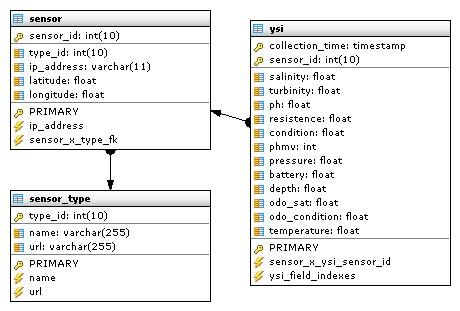
\includegraphics[scale=0.65]{../diagrams/Relational-Model-Original}
  \caption{Relational Data Model for NetBEAMS - A first prototype}
  \label{fig:Relational-Model-Original}
\end{figure}

Supposing a new type is added into the system, let the refactored
version of the relational model be depicted in figure
\ref{fig:Relational-Model-Addition-Modified}.

\begin{figure}
  \centering
  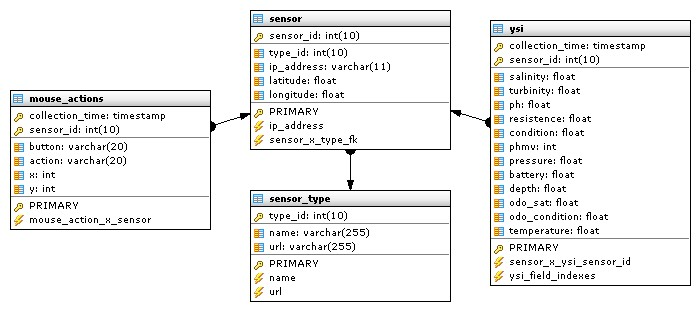
\includegraphics[scale=0.65]{../diagrams/Relational-Model-Addition-Modified}
  \caption{Relational Data Model for NetBEAMS - Modified version with new
  entity}
  \label{fig:Relational-Model-Addition-Modified}
\end{figure}

\begin{itemize}
  \item Constant data schema changes require constant database normalization
  process, changes to structure, database management, etc;
  \item Some research have shown that the Relational Model does not fit the
  nature of collected data from wired or wireless sensor networks. They usually
  does not support time-series data nor provenance.
  \item Even project aiming at updating the relational sensor database systems
  and SQL clauses have been proposed. 
\end{itemize}

Other projects have been using the XML data models. It falls into the same
category as the Relational Model, since the XML documents, when in the context
of a database, must be complaint to an XML Schema. As shown in section 3, this
model uses XPath technology for querying documents, although some hibrid
technologies may still use SQL for that matter. In this way, an instance of
such schema dependent types can be seen in figure
\ref{fig:persistence-example-relational}.

\begin{figure}[!h]
  \centering
  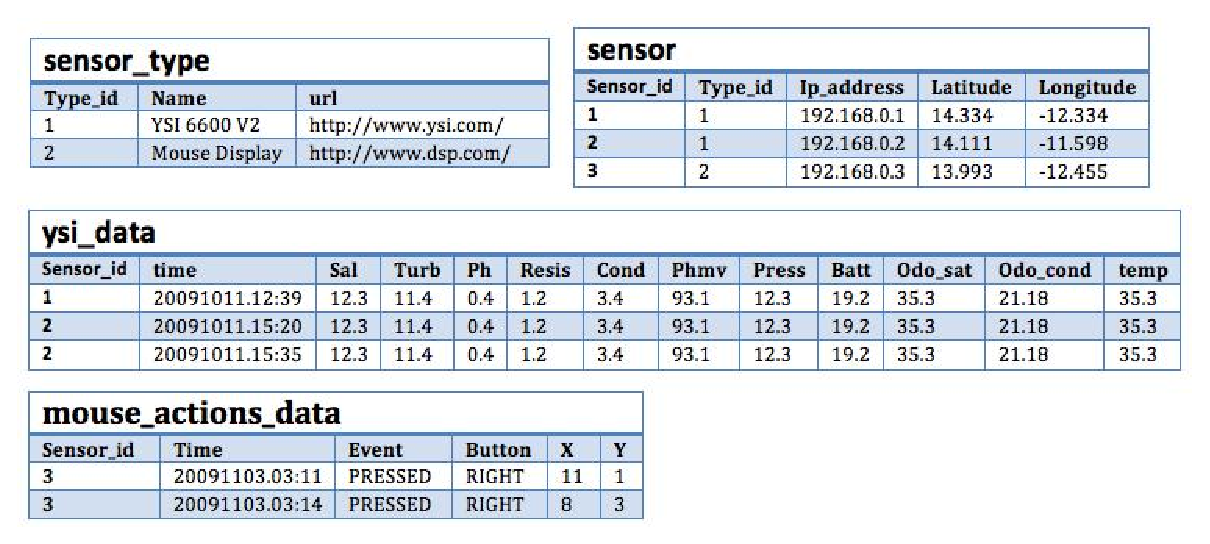
\includegraphics[scale=0.65]{../diagrams/persistence-example-relational}
  \caption{Instance of a Relational Model Database Prototype}
  \label{fig:persistence-example-relational}
\end{figure}

Although this data model have been used in different types of applications,
developers have tried to use the Relational Model to model an application that
could prevent any database change through the use of a technique that relates a
key to a value, called Key-Value data model. With the advent of Internet
applications, the need of such a model that does not need constant refactoring
led developers to propose such approach using the relational model as
documented in technical articles such as \cite{db-kvp-in-relational01} and
\cite{db-kvp-in-relational02}. Based in these articles, consider the relational
model depicted in figure \ref{fig:KVP-on-Relational-Model} as model for the
persistence data for our case study using the key-value strategy. The problem
with it is that key repetition occurs, since the nature of time-series data
requires the use of a timestamp key for each property of the sensor. Therefore,
this strategy is not well-suited to provide persistence data from collected
sensor networks.

\begin{figure}[!h]
  \centering
  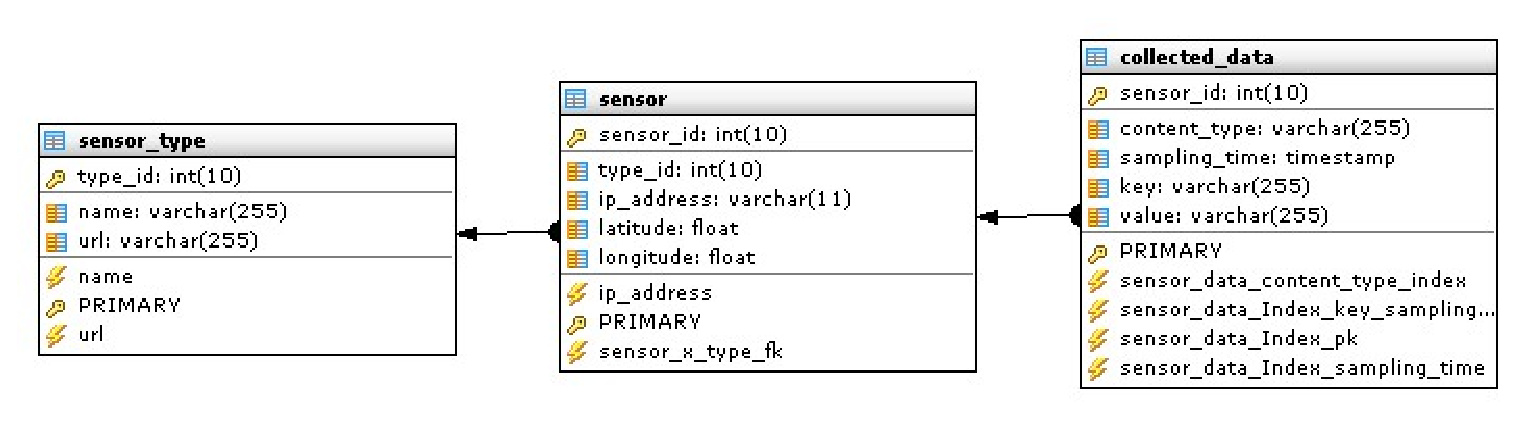
\includegraphics[scale=0.5]{../diagrams/KVP-on-Relational-Model}
  \caption{KVP Data Model implementation using Relational Model}
  \label{fig:KVP-on-Relational-Model}
\end{figure}

\begin{figure}[!h]
  \centering
  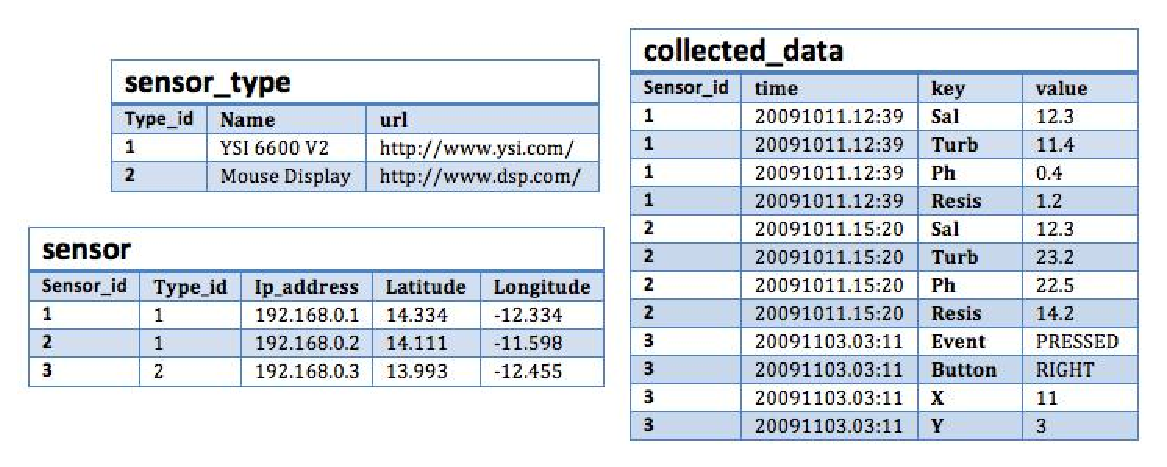
\includegraphics[scale=0.5]{../diagrams/persistence-example-relational-kvp}
  \caption{KVP over Relational Model Database Prototype}
  \label{fig:persistence-example-relational-kvp}
\end{figure}

\subsection{Analysis of the Schema-less Models}

The advance of Cloud Computing, and dynamic web applications have motivated the
database community to implement different mechanisms for persisting data
without the heavy-process of data modeling. Given the fact that sensor networks
may be updated at any time by the addition of new sensor types, the use of
moding approaches such as Key-Value Database have been proposed \cite{db-kvp}.

\begin{itemize}
  \item entities from the same domains are placed into a bucket;
  \item entities have a set of attributes and relating values
  \item entities with different set of attributes may be contained in the same
  bucket, since there is no schema to govern the bucket items restriction.
\end{itemize}

For instance, all data needed for the YSI sonde data, as well as all necessary
provenance data that describes the data, are represented by means of key-value
pairs \ref{fig:persistence-example-kvp}.

\begin{figure}[!h]
  \centering
  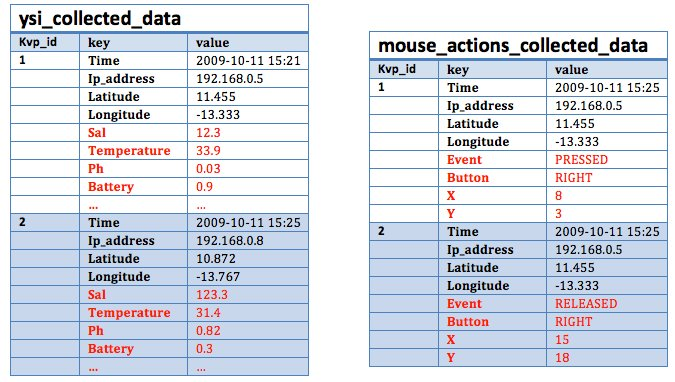
\includegraphics[scale=0.5]{../diagrams/persistence-example-kvp}
  \caption{KVP Database instance Prototype}
  \label{fig:persistence-example-kvp}
\end{figure}

\subsection{Technology Analysis}

The data models were compared by \cite{db-is-rdbs-dommed} and can be summarized
as follows:

\begin{table}
    \label{tab:ysi-data-distribution}
    \caption{Schema-Dependent X Schema-less Databases Compared: Properties}
    \begin{center}
    \begin{tabular}{|p{210pt}|p{210pt}|}\hline
    Schema-Dependent Databases & Schema-less Databases\\\hline
    \begin{enumerate}
      \item Real-world model by entities, classified in tables;
      \item Tables composed by columns and rows. Rows are comprised by column
      values, which have the same schema;
      \item Data Model defined in advance with a schema, which contains
      relationships and constraints to enforce data integrity;
      \item Data represents ``natural'' entities, not application specific;
      \item Data Normalization is the data structuring process to remove data
      duplication, as well as establishing data associations through table
      relationships.
    \end{enumerate} 
    & 
    \begin{enumerate}
      \item Real-world model by entities, classified in Domains;
      \item Domains are similar to tables, but like buckets that contains items
      without a pre-defined schema, what enable them to have different schemas;
      \item Items are identified by keys, as well as have a dynamic set of
      attributes attached to it, however with no schema defined;
      \item Items may represent not only the natural representation of data, but
      also include application-specific data;
      \item Since data may be repeated, no data normalization is done, so that
      integrity is done in the application layer.
    \end{enumerate}
    \\\hline
    \end{tabular}
    \end{center}
\end{table}

\begin{table}
    \label{tab:ysi-data-distribution}
    \caption{Schema-Dependent X Schema-less Databases: Data Access}
    \begin{center}
    \begin{tabular}{|p{210pt}|p{210pt}|}\hline
    Schema-Dependent Databases & Schema-less Databases\\\hline
    \begin{enumerate}
      \item The basic operations CRUD \footnote{Create-Retrieve-Update-Update
      database operations} data are performed using a structured language such
      as the SQL or XPath;
      \item Query languages can access data from different tables through
      joins, contains functions for aggregation and complex filter.
    \end{enumerate} 
    & 
    \begin{enumerate}
      \item The CRUD operations are performed via API \footnote{Application
      Programming Interface} through programming languages;
      \item Some technologies provide basic SQL-like syntax for filter criteria
      with some predicates like =, !=, <, > that ca be applied;
      \item The data and application integrity logic is placed in the
      application layer.
    \end{enumerate}
    \\\hline
    \end{tabular}
    \end{center}
\end{table}

\begin{table}
    \label{tab:ysi-data-distribution}
    \caption{Schema-Dependent X Schema-less Databases: Application Interface}
    \begin{center}
    \begin{tabular}{|p{210pt}|p{210pt}|}\hline
    Schema-Dependent Databases & Schema-less Databases\\\hline
    \begin{enumerate}
      \item Have their own specific API or through ODBC\footnote{Open Database
      Connectivity};
      \item Data is stored in a format that represents its natural structure,
      and for this reason, in a single or distributed fashion.
    \end{enumerate} 
    & 
    \begin{enumerate}
      \item Systems tend to provide SOAP/REST \cite{http-rest};
      \item \cite{db-is-rdbs-dommed} claims that data is stored in a more
      effective way, requiring only code plumbing for the relational code;
    \end{enumerate}
    \\\hline
    \end{tabular}
    \end{center}
\end{table}

\begin{itemize}
  \item MySQL: NO SUPPORT
  \item Microsoft SQL: NO SUPPORT
  \item Berkeley TinyDB: NO SUPPORT
  \item \textbf{MongoDB}: Supports Both
  \item \textbf{CouchDB}: Supports Both
  \item IBM DB2: NO SUPPORT
\end{itemize}

\section{Analysis of the Database System Organization Taxonomy}

Sensor Network data can be saved in either Centralized or Distributed Systems.
While Centralized Database Systems are easier to manage, it may face challenges
regarding its data. For this reason, the use of partitioning or sharding would
be an addition to persist sensor data.

\subsection{Advantages of Database Partitioning and Sharding}

\begin{itemize}
  \item Data-Centric queries and data use;
  \item Solves bottleneck problems related to reads/writes;
  \item Decrease the funneling effect by directing queries to given data
  partition;
\end{itemize}

\subsection{Disadvantages of Database Partitioning and Sharding}

\begin{itemize}
  \item Very advanced topics in Database System;
  \item May be easy of use, depending on the application.
\end{itemize}

\subsection{Technology Analysis}

\begin{itemize}
  \item \textbf{MySQL}: Supports
  \item \textbf{Microsoft SQL}: Supports
  \item \textbf{Berkeley TinyDB}: NO Supports
  \item \textbf{MongoDB}: Supports
  \item \textbf{CouchDB}: Supports
  \item \textbf{IBM DB2}: Supports
\end{itemize}

\section{Other Non-Functional Analysis}

\begin{itemize}
  \item Given the fact of the nature of the project, the technology to be used
  must be \textbf{open-source} \cite{open-source}, that is, no costs involved
  in the adoption of such technology;
  \item A solution for persisting collected sensor data must be not only limited
  to a technology that provides data access, such as SQL, but also by other
  \textbf{data access mechanisms} such as through \textbf{native APIs}. The
  reason is that part of the sensor network data does not have skills in
  database models, but may have skills with programming languages;
  \item Supports hot backup without service interruption.
\end{itemize}

\subsection{Technology Analysis}

Most of the technologies listed provides access to the data sets through the
use of drivers in different programming and scripting languages such as Java,
Python, Perl, etc.

\begin{itemize}
  \item \textbf{MySQL}: Supports
  \item \textbf{Microsoft SQL}: Supports
  \item \textbf{Berkeley TinyDB}: Supports
  \item \textbf{MongoDB}: Supports
  \item \textbf{CouchDB}: Supports
  \item \textbf{IBM DB2}: Supports
\end{itemize}

\section{Global Analysis Results and Technology Selection}

\begin{table}
    \label{tab:ysi-data-distribution}
    \caption{Amount of data produced by the RTC's YSI sondes}
        \begin{center}
        \begin{tabular}{|c|c|c|c|c|c|c|}\hline 
        \textbf{Database} & \textbf{MySQL} & \textbf{MicrosoftSQL} & \textbf{TinyDB} &
        \textbf{MongoDB} & \textbf{CouchDB} & \textbf{IBM DB2}\\\hline 
        Centralized Query & + & + & + & + & + & + \\\hline 
        Distributed System & ++ & ++ & - & ++ & ++ & +\\\hline 
        Schema-less & - & - & - & + & + & +\\\hline 
        Provenance Support & + & + & + & + & + & +\\\hline 
        NO-SQL Query & - & - & - & + & + & +\\\hline 
        Data Partition & + & + & - & + & + & +\\\hline 
        Hot Backup & + & + & - & - & - & +\\\hline 
        Export Capability & + & + & - & + & + & -\\\hline 
        Programming Lang. & + & + & + & + & + & +\\\hline
        Script Lang. & + & + & - & + & + & +\\\hline
        Open-Source & + & - & + & + & + & -\\\hline
        \end{tabular}
        \end{center}
\end{table}
